% !TEX encoding = UTF-8 Unicode
% !TEX TS-program = xelatex
\begin{QUESTIONS}
    \begin{QUESTION}
        \begin{ExamInfo}{103}{學測}{單選}{1}
        \end{ExamInfo}
        \begin{ExamAnsRateInfo}{82}{99}{93}{54}
        \end{ExamAnsRateInfo}
        \begin{QBODY}
            請問下列哪一個選項等於$\log \left( {{2}^{\left( {{3}^{5}} \right)}} \right)$?
			\begin{QOPS}
				\QOP $5\log \left( {{2}^{3}} \right)$
				\QOP $3\times 5\log 2$
				\QOP $5\log 2\times \log 3$
				\QOP $5\left( \log 2+\log 3 \right)$
				\QOP ${{3}^{5}}\log 2$
			\end{QOPS}
        \end{QBODY}
        \begin{QFROMS}
        \end{QFROMS}
        \begin{QTAGS}\QTAG{B1C3-3對數}\QTAG{B1C3指對數函數}\QTAG{對數律}\end{QTAGS}
        \begin{QANS}
            (5)
        \end{QANS}
        \begin{QSOLLIST}
        \end{QSOLLIST}
        \begin{QEMPTYSPACE}
        \end{QEMPTYSPACE}
    \end{QUESTION}
    \begin{QUESTION}
        \begin{ExamInfo}{103}{學測}{單選}{2}
        \end{ExamInfo}
        \begin{ExamAnsRateInfo}{74}{95}{85}{42}
        \end{ExamAnsRateInfo}
        \begin{QBODY}
            令$A(5,0,12)$、$B(-5,0,12)$為坐標空間中之兩點,且令$P$為$xy$平面上滿足$\overline{PA}=\overline{PB}=13$的點。請問下列哪一個選項中的點可能為$P$?
			\begin{QOPS}
				\QOP $(5,0,0)$
				\QOP $(5,5,0)$
				\QOP $(0,12,0)$
				\QOP $(0,0,0)$
				\QOP $(0,0,24)$
			\end{QOPS}
        \end{QBODY}
        \begin{QFROMS}
        \end{QFROMS}
        \begin{QTAGS}\QTAG{B4C1-2空間向量的坐標表示法}\QTAG{B4C1空間向量}\end{QTAGS}
        \begin{QANS}
            (4)
        \end{QANS}
        \begin{QSOLLIST}
        \end{QSOLLIST}
        \begin{QEMPTYSPACE}
        \end{QEMPTYSPACE}
    \end{QUESTION}
    \begin{QUESTION}
        \begin{ExamInfo}{103}{學測}{單選}{3}
        \end{ExamInfo}
        \begin{ExamAnsRateInfo}{73}{96}{86}{37}
        \end{ExamAnsRateInfo}
        \begin{QBODY}
            3.	在坐標平面上,以$(1,1),\ (-1,1),\ (-1,-1)$及$(1,-1)$等四個點為頂點的正方形,與圓${{x}^{2}}+{{y}^{2}}+2x+2y+1=0$有幾個交點?
			\begin{QOPS}
				\QOP 1個
				\QOP 2個
				\QOP 3個
				\QOP 4個
				\QOP 0個
			\end{QOPS}
        \end{QBODY}
        \begin{QFROMS}
        \end{QFROMS}
        \begin{QTAGS}\QTAG{B3C2-3圓與直線的關係}\QTAG{B3C2直線與圓}\end{QTAGS}
        \begin{QANS}
            (2)
        \end{QANS}
        \begin{QSOLLIST}
        \end{QSOLLIST}
        \begin{QEMPTYSPACE}
        \end{QEMPTYSPACE}
    \end{QUESTION}
    \begin{QUESTION}
        \begin{ExamInfo}{103}{學測}{單選}{4}
        \end{ExamInfo}
        \begin{ExamAnsRateInfo}{68}{95}{79}{30}
        \end{ExamAnsRateInfo}
        \begin{QBODY}
            請問滿足絕對值不等式$\left| 4x-12 \right|\le 2x$的實數$x$所形成的區間,其長度為下列哪一個選項?
			\begin{QOPS}
				\QOP 1
				\QOP 2
				\QOP 3
				\QOP 4
				\QOP 6
			\end{QOPS}
        \end{QBODY}
        \begin{QFROMS}
        \end{QFROMS}
        \begin{QTAGS}\QTAG{B1C1數與式}\end{QTAGS}
        \begin{QANS}
            (4)
        \end{QANS}
        \begin{QSOLLIST}
        \end{QSOLLIST}
        \begin{QEMPTYSPACE}
        \end{QEMPTYSPACE}
    \end{QUESTION}
    \begin{QUESTION}
        \begin{ExamInfo}{103}{學測}{單選}{5}
        \end{ExamInfo}
        \begin{ExamAnsRateInfo}{69}{97}{77}{33}
        \end{ExamAnsRateInfo}
        \begin{QBODY}
            設${{(1+\sqrt{2})}^{6}}=a+b\sqrt{2}$,其中$a,b$為整數。請問b等於下列哪一個選項?
			\begin{QOPS}
				\QOP $C_{0}^{6}+2C_{2}^{6}+{{2}^{2}}C_{4}^{6}+{{2}^{3}}C_{6}^{6}$
				\QOP $C_{1}^{6}+2C_{3}^{6}+{{2}^{2}}C_{5}^{6}$
				\QOP $C_{0}^{6}+2C_{1}^{6}+{{2}^{2}}C_{2}^{6}+{{2}^{3}}C_{3}^{6}+{{2}^{4}}C_{4}^{6}+{{2}^{5}}C_{5}^{6}+{{2}^{6}}C_{6}^{6}$
				\QOP $2C_{1}^{6}+{{2}^{2}}C_{3}^{6}+{{2}^{3}}C_{5}^{6}$
				\QOP $C_{0}^{6}+{{2}^{2}}C_{2}^{6}+{{2}^{4}}C_{4}^{6}+{{2}^{6}}C_{6}^{6}$
			\end{QOPS}
        \end{QBODY}
        \begin{QFROMS}
        \end{QFROMS}
        \begin{QTAGS}\QTAG{B2C2-4二項式定理}\QTAG{B2C2排列組合}\end{QTAGS}
        \begin{QANS}
            (2)
        \end{QANS}
        \begin{QSOLLIST}
        \end{QSOLLIST}
        \begin{QEMPTYSPACE}
        \end{QEMPTYSPACE}
    \end{QUESTION}
    \begin{QUESTION}
        \begin{ExamInfo}{103}{學測}{單選}{6}
        \end{ExamInfo}
        \begin{ExamAnsRateInfo}{33}{55}{22}{22}
        \end{ExamAnsRateInfo}
        \begin{QBODY}
            某疾病可分為兩種類型:第一類占$70\%$,可藉由藥物$A$治療,其每一次療程的成功率為$70\%$,且每一次療程的成功與否互相獨立;其餘為第二類,藥物$A$治療方式完全無效。在不知道患者所患此疾病的類型,且用藥物$A$第一次療程失敗的情況下,進行第二次療程成功的條件機率最接近下列哪一個選項?
                \begin{QOPS}
    				\QOP $0.25$
    				\QOP $0.3$
    				\QOP $0.35$
    				\QOP $0.4$
    				\QOP $0.45$
                \end{QOPS}
        \end{QBODY}
        \begin{QFROMS}
        \end{QFROMS}
        \begin{QTAGS}\QTAG{B2C3機率}\QTAG{B2C3-3條件機率與貝氏定理}\end{QTAGS}
        \begin{QANS}
            (2)
        \end{QANS}
        \begin{QSOLLIST}
        \end{QSOLLIST}
        \begin{QEMPTYSPACE}
        \end{QEMPTYSPACE}
    \end{QUESTION}
\end{QUESTIONS}
\begin{QUESTIONS}
    \begin{QUESTION}
        \begin{ExamInfo}{103}{學測}{多選}{7}
        \end{ExamInfo}
        \begin{ExamAnsRateInfo}{62}{89}{65}{32}
        \end{ExamAnsRateInfo}
        \begin{QBODY}
            設坐標平面上,x坐標與y坐標皆為整數的點稱為格子點。請選出圖形上有格子點的選項。
			\begin{QOPS}
				\QOP $y={{x}^{2}}$
				\QOP $3y=9x+1$
				\QOP ${{y}^{2}}=-x-2$
				\QOP ${{x}^{2}}+{{y}^{2}}=3$
				\QOP $y={{\log }_{9}}x+\frac{1}{2}$
			\end{QOPS}
        \end{QBODY}
        \begin{QFROMS}
        \end{QFROMS}
        \begin{QTAGS}\QTAG{跨章節試題}\end{QTAGS}
        \begin{QANS}
            (1)(3)(5)
        \end{QANS}
        \begin{QSOLLIST}
        \end{QSOLLIST}
        \begin{QEMPTYSPACE}
        \end{QEMPTYSPACE}
    \end{QUESTION}
    \begin{QUESTION}
        \begin{ExamInfo}{103}{學測}{多選}{8}
        \end{ExamInfo}
        \begin{ExamAnsRateInfo}{73}{92}{82}{45}
        \end{ExamAnsRateInfo}
        \begin{QBODY}
            關於下列不等式,請選出正確的選項。
			\begin{QOPS}
				\QOP $\sqrt{13}>3.5$
				\QOP $\sqrt{13}<3.6$
				\QOP $\sqrt{13}-\sqrt{3}>\sqrt{10}$
				\QOP $\sqrt{13}+\sqrt{3}>\sqrt{16}$
				\QOP $\frac{1}{\sqrt{13}-\sqrt{3}}>0.6$
			\end{QOPS}
        \end{QBODY}
        \begin{QFROMS}
        \end{QFROMS}
        \begin{QTAGS}\QTAG{B1C1數與式}\end{QTAGS}
        \begin{QANS}
            (1)(4)
        \end{QANS}
        \begin{QSOLLIST}
        \end{QSOLLIST}
        \begin{QEMPTYSPACE}
        \end{QEMPTYSPACE}
    \end{QUESTION}
    \begin{QUESTION}
        \begin{ExamInfo}{103}{學測}{多選}{9}
        \end{ExamInfo}
        \begin{ExamAnsRateInfo}{71}{94}{77}{42}
        \end{ExamAnsRateInfo}
        \begin{QBODY}
            一物體由坐標平面中的點$(-3,6)$出發,沿著向量$\lvec{v}$所指的方向持續前進,可以進入第一象限。請選出正確的選項。
			\begin{QOPS}
				\QOP $\lvec{v}=(1,-2)$
				\QOP $\lvec{v}=(1,-1)$
				\QOP $\lvec{v}=(0.001,0)$
				\QOP $\lvec{v}=(0.001,1)$
				\QOP $\lvec{v}=(-0.001,1)$
			\end{QOPS}
        \end{QBODY}
        \begin{QFROMS}
        \end{QFROMS}
        \begin{QTAGS}\QTAG{B3C3-1平面向量的表示法}\QTAG{B3C3平面向量}\end{QTAGS}
        \begin{QANS}
            (2)(3)(4)
        \end{QANS}
        \begin{QSOLLIST}
        \end{QSOLLIST}
        \begin{QEMPTYSPACE}
        \end{QEMPTYSPACE}
    \end{QUESTION}
    \begin{QUESTION}
        \begin{ExamInfo}{103}{學測}{多選}{10}
        \end{ExamInfo}
        \begin{ExamAnsRateInfo}{53}{83}{52}{24}
        \end{ExamAnsRateInfo}
        \begin{QBODY}
            設$f(x)$為實係數二次多項式,且已知$f(1)>0$、$f(2)<0$、$f(3)>0$。
		令$g(x)=f(x)+(x-2)(x-3)$,請選出正確的選項。
		\begin{QOPS}
			\QOP $y=f(x)$的圖形是開口向下的拋物線
			\QOP $y=g(x)$的圖形是開口向下的拋物線
			\QOP $g(1)>f(1)$
			\QOP $g(x)=0$在1與2之間恰有一個實根
			\QOP 若$\alpha $為$f(x)=0$的最大實根,則$g(\alpha )>0$
		\end{QOPS}
        \end{QBODY}
        \begin{QFROMS}
        \end{QFROMS}
        \begin{QTAGS}\QTAG{B1C2多項式函數}\QTAG{B1C2-3多項式方程式}\QTAG{圖形}\QTAG{二次多項式}\QTAG{勘根定理}\end{QTAGS}
        \begin{QANS}
            (3)(4)
        \end{QANS}
        \begin{QSOLLIST}
        \end{QSOLLIST}
        \begin{QEMPTYSPACE}
        \end{QEMPTYSPACE}
    \end{QUESTION}
    \begin{QUESTION}
        \begin{ExamInfo}{103}{學測}{多選}{11}
        \end{ExamInfo}
        \begin{ExamAnsRateInfo}{50}{80}{50}{20}
        \end{ExamAnsRateInfo}
        \begin{QBODY}
            設${{a}_{1}}=1$且${{a}_{1}},{{a}_{2}},{{a}_{3}},\ldots $為等差數列。請選出正確的選項。
			\begin{QOPS}
				\QOP 若${{a}_{100}}>0$,則${{a}_{1000}}>0$
				\QOP 若${{a}_{100}}<0$,則${{a}_{1000}}<0$
				\QOP 若${{a}_{1000}}>0$,則${{a}_{100}}>0$
				\QOP 若${{a}_{1000}}<0$,則${{a}_{100}}<0$
				\QOP ${{a}_{1000}}-{{a}_{10}}=10\,({{a}_{100}}-{{a}_{1}})$
			\end{QOPS}
        \end{QBODY}
        \begin{QFROMS}
        \end{QFROMS}
        \begin{QTAGS}\QTAG{B2C1數列級數}\QTAG{B2C1-1數列}\QTAG{等差數列}\end{QTAGS}
        \begin{QANS}
            (2)(3)(5)
        \end{QANS}
        \begin{QSOLLIST}
        \end{QSOLLIST}
        \begin{QEMPTYSPACE}
        \end{QEMPTYSPACE}
    \end{QUESTION}
    \begin{QUESTION}
        \begin{ExamInfo}{103}{學測}{多選}{12}
        \end{ExamInfo}
        \begin{ExamAnsRateInfo}{44}{67}{40}{25}
        \end{ExamAnsRateInfo}
        \begin{QBODY}
            所謂某個年齡範圍的失業率,是指該年齡範圍的失業人數與勞動力人數之比,以百分數表達(進行統計分析時,所有年齡以整數表示)。下表為去年某國四個年齡範圍的失業率,\underline{\textbf{其中的年齡範圍有所重疊}}。
			\begin{tabular}{c|c|c|c|c}
			年齡範圍  & 	35~44歲	& 35~39歲	 & 40~44歲	     & 45~49歲     \\\hline 
			失業率	  & $12.66(\%)$	& $9.80(\%)$ &	$13.17(\%)$	 & $7.08(\%)$    
			\end{tabular}
        \end{QBODY}
        \begin{QFROMS}
        \end{QFROMS}
        \begin{QTAGS}\QTAG{B2C4-1一維數據分析}\QTAG{B2C4數據分析}\QTAG{加權平均數}\end{QTAGS}
        \begin{QANS}
            (1)(4)
        \end{QANS}
        \begin{QSOLLIST}
        \end{QSOLLIST}
        \begin{QEMPTYSPACE}
        \end{QEMPTYSPACE}
    \end{QUESTION}
\end{QUESTIONS}
\begin{QUESTIONS}
    \begin{QUESTION}
        \begin{ExamInfo}{103}{學測}{填充}{A}
        \end{ExamInfo}
        \begin{ExamAnsRateInfo}{64}{97}{78}{17}
        \end{ExamAnsRateInfo}
        \begin{QBODY}
            設圓$O$之半徑為$24$,$\overline{OC}=26$,$\overline{OC}$交圓$O$於$A$點,$\overline{CD}$切圓$O$於$D$點,$B$為$A$點到$\overline{OD}$的垂足,如右邊的示意圖。則$\overline{AB}=\TCNBOX{\FR{\TCN\TCN\TCN}{\TCN\TCN}}$
			
			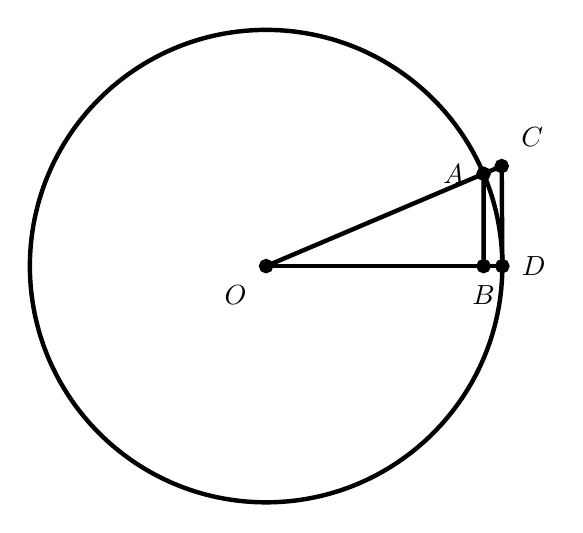
\begin{tikzpicture}[scale=1.5] 
				\coordinate (O) at (0:0);
				\coordinate (A) at (23:2);
				\coordinate (C) at (23:{13/6});

				\coordinate (yaxis) at (0,2);
				\coordinate (xaxis) at (2,0);
				\coordinate (D) at (2,0);
				\coordinate (B) at (xaxis -| A);
				
				\draw[ultra thick] (0,0) circle (2);
				\draw [ultra thick] (O) -- (C);
				\draw [ultra thick] (O) -- (D);
				\draw [ultra thick] (C) -- (D);
				\draw [ultra thick] (A) -- (B);

				\foreach \v/\u/\t in 
				{   A/180/$A$,
					B/270/$B$,
					C/45/$C$,
					D/0/$D$,
					O/225/$O$
				}
				{
					\draw[ultra thick,fill] (\v) circle (1.2pt);
					\node[label=\u:\t] at (\v){};
				};
				
			\end{tikzpicture}
        \end{QBODY}
        \begin{QFROMS}
        \end{QFROMS}
        \begin{QTAGS}\QTAG{B3C1三角}\QTAG{B3C1-2廣義角與極坐標}\end{QTAGS}
        \begin{QANS}
            $\dfrac{120}{13}$
        \end{QANS}
        \begin{QSOLLIST}
        \end{QSOLLIST}
        \begin{QEMPTYSPACE}
        \end{QEMPTYSPACE}
    \end{QUESTION}
    \begin{QUESTION}
        \begin{ExamInfo}{103}{學測}{填充}{B}
        \end{ExamInfo}
        \begin{ExamAnsRateInfo}{15}{42}{3}{0}
        \end{ExamAnsRateInfo}
        \begin{QBODY}
            坐標平面上,若直線$y=ax+b$(其中$a,b$為實數)與二次函數$y={{x}^{2}}$的圖形恰交於一點,亦與二次函數$y={{(x-2)}^{2}}+12$的圖形恰交於一點,則$a=\TCNBOX{TCN}$,$b=\TCNBOX{\TCN\TCN}$。
        \end{QBODY}
        \begin{QFROMS}
        \end{QFROMS}
        \begin{QTAGS}\QTAG{一次多項式}\QTAG{B1C2多項式函數}\QTAG{圖形}\QTAG{二次多項式}\QTAG{B1C2-1簡單的多項式及圖形}\end{QTAGS}
        \begin{QANS}
            $6$, $-9$
        \end{QANS}
        \begin{QSOLLIST}
        \end{QSOLLIST}
        \begin{QEMPTYSPACE}
        \end{QEMPTYSPACE}
    \end{QUESTION}
    \begin{QUESTION}
        \begin{ExamInfo}{103}{學測}{填充}{C}
        \end{ExamInfo}
        \begin{ExamAnsRateInfo}{49}{87}{53}{7}
        \end{ExamAnsRateInfo}
        \begin{QBODY}
            小鎮A距離一筆直道路6公里,並與道路上的小鎮B相距12公里。今欲在此道路上蓋一家超級市場使其與A, B等距,則此超級市場與A的距離須為$\TCNBOX{\TCN\sqrt{\TCN}}$公里。(化為最簡根式)
        \end{QBODY}
        \begin{QFROMS}
        \end{QFROMS}
        \begin{QTAGS}\QTAG{B3C2-1直線方程式及其圖形}\QTAG{B3C2直線與圓}\end{QTAGS}
        \begin{QANS}
            $4\sqrt{3}$
        \end{QANS}
        \begin{QSOLLIST}
        \end{QSOLLIST}
        \begin{QEMPTYSPACE}
        \end{QEMPTYSPACE}
    \end{QUESTION}
    \begin{QUESTION}
        \begin{ExamInfo}{103}{學測}{填充}{D}
        \end{ExamInfo}
        \begin{ExamAnsRateInfo}{31}{76}{16}{1}
        \end{ExamAnsRateInfo}
        \begin{QBODY}
            坐標空間中有四點$A(2,0,0)$、$B(3,4,2)$、$C(-2,4,0)$與$D(-1,3,1)$。若點$P$在直線$CD$上變動,則內積$\lvec{PA}\cdot \lvec{PB}$ 之最小可能值為 $\TCNBOX{\FR{\TCN}{\TCN}}$。(化為最簡分數)
        \end{QBODY}
        \begin{QFROMS}
        \end{QFROMS}
        \begin{QTAGS}\QTAG{B4C2-2空間直線方程式}\QTAG{B4C2空間中的平面與直線}\QTAG{參數式}\end{QTAGS}
        \begin{QANS}
            $\dfrac{5}{4}$
        \end{QANS}
        \begin{QSOLLIST}
        \end{QSOLLIST}
        \begin{QEMPTYSPACE}
        \end{QEMPTYSPACE}
    \end{QUESTION}
    \begin{QUESTION}
        \begin{ExamInfo}{103}{學測}{填充}{E}
        \end{ExamInfo}
        \begin{ExamAnsRateInfo}{31}{75}{17}{1}
        \end{ExamAnsRateInfo}
        \begin{QBODY}
            設$\lvec{u},\lvec{v}$為兩個長度皆為$1$的向量。若$\lvec{u} +\lvec{v}$ 與u的夾角為$75{}^\circ $,則$\lvec{u}$與$\lvec{v} $的內積為$\TCNBOX{\FR{\TCN\sqrt{\TCN}}{\TCN}}$。(化為最簡根式)
        \end{QBODY}
        \begin{QFROMS}
        \end{QFROMS}
        \begin{QTAGS}\QTAG{線性組合}\QTAG{B3C3-2平面向量的內積}\QTAG{B3C3-1平面向量的表示法}\QTAG{B3C3平面向量}\QTAG{夾角}\end{QTAGS}
        \begin{QANS}
            $-\dfrac{\sqrt{3}}{2}$
        \end{QANS}
        \begin{QSOLLIST}
        \end{QSOLLIST}
        \begin{QEMPTYSPACE}
        \end{QEMPTYSPACE}
    \end{QUESTION}
    \begin{QUESTION}
        \begin{ExamInfo}{103}{學測}{填充}{F}
        \end{ExamInfo}
        \begin{ExamAnsRateInfo}{22}{44}{17}{5}
        \end{ExamAnsRateInfo}
        \begin{QBODY}
            一個房間的地面是由$12$個正方形所組成,如右圖。今想用長方形瓷磚舖滿地面,已知每一塊長方形瓷磚可以覆蓋兩個相鄰的正方形,即
			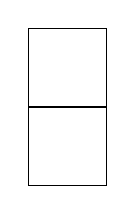
\begin{tikzpicture}[scale=1]
				\draw[color=black] (0,0) grid (1,2);
			\end{tikzpicture} 
			或 
			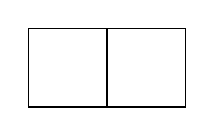
\begin{tikzpicture}[scale=1]
				\draw[color=black] (0,0) grid (2,1);
			\end{tikzpicture}。
			則用$6$塊瓷磚舖滿房間地面的方法有$\TCNBOX{\TCN}{\TCN}$種

			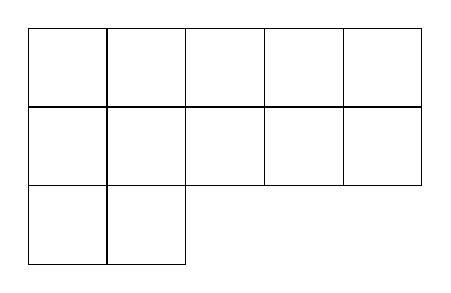
\begin{tikzpicture}[scale=1]
				\draw[color=black] (0,0) grid (2,3);
				\draw[color=black] (2,1) grid (5,3);
			\end{tikzpicture}
        \end{QBODY}
        \begin{QFROMS}
        \end{QFROMS}
        \begin{QTAGS}\QTAG{B2C1數列級數}\QTAG{乘法原理加法原理}\QTAG{B2C1-1數列}\QTAG{B2C2排列組合}\QTAG{遞迴}\end{QTAGS}
        \begin{QANS}
            $11$
        \end{QANS}
        \begin{QSOLLIST}
        \end{QSOLLIST}
        \begin{QEMPTYSPACE}
        \end{QEMPTYSPACE}
    \end{QUESTION}
    \begin{QUESTION}
        \begin{ExamInfo}{103}{學測}{填充}{G}
        \end{ExamInfo}
        \begin{ExamAnsRateInfo}{35}{76}{25}{4}
        \end{ExamAnsRateInfo}
        \begin{QBODY}
            已知$\left[ \begin{matrix}
   a & b  \\
   c & d  \\
\end{matrix} \right]$是一個轉移矩陣,並且其行列式(值)為$\frac{5}{8}$。則$a+d=\TCNBOX{\TCN\TCN}{\TCN}$。(化為最簡分數)
        \end{QBODY}
        \begin{QFROMS}
        \end{QFROMS}
        \begin{QTAGS}\QTAG{馬可夫鍊}\QTAG{B4C3矩陣}\QTAG{B4C3-3矩陣的應用}\end{QTAGS}
        \begin{QANS}
            $\dfrac{13}{8}$
        \end{QANS}
        \begin{QSOLLIST}
        \end{QSOLLIST}
        \begin{QEMPTYSPACE}
        \end{QEMPTYSPACE}
    \end{QUESTION}
    \begin{QUESTION}
        \begin{ExamInfo}{103}{學測}{填充}{H}
        \end{ExamInfo}
        \begin{ExamAnsRateInfo}{28}{64}{18}{2}
        \end{ExamAnsRateInfo}
        \begin{QBODY}
            %TOOD:補圖
			如圖,正三角形$ABC$的邊長為1,並且$\angle 1=\angle 2=\angle 3=15{}^\circ $。已知$\sin 15{}^\circ =\frac{\sqrt{6}-\sqrt{2}}{4}$,則正三角形$DEF$的邊長為$\TCNBOX{\FR{\sqrt{\TCN}}{\TCN}-\FR{\sqrt{\TCN}}{\TCN}}$。(化為最簡根式)
        \end{QBODY}
        \begin{QFROMS}
        \end{QFROMS}
        \begin{QTAGS}\QTAG{B3C1-4差角公式}\QTAG{B3C1三角}\end{QTAGS}
        \begin{QANS}
            $\dfrac{\sqrt{6}}{2}-\dfrac{\sqrt{2}}{2}$
        \end{QANS}
        \begin{QSOLLIST}
        \end{QSOLLIST}
        \begin{QEMPTYSPACE}
        \end{QEMPTYSPACE}
    \end{QUESTION}
\end{QUESTIONS}
